\documentclass[12pt,notitlepage,letterpaper]{article}
\usepackage[margin=0.5in]{geometry}
\usepackage[utf8]{inputenc}
\usepackage{amsmath,amsfonts,amssymb,graphicx}
\usepackage{tikz}

\begin{document}
\title{Inter-Device Sharing}
\date{}
\maketitle

\section{Overview}

\section{Sharing flow between UI and backend}
\begin{figure}
    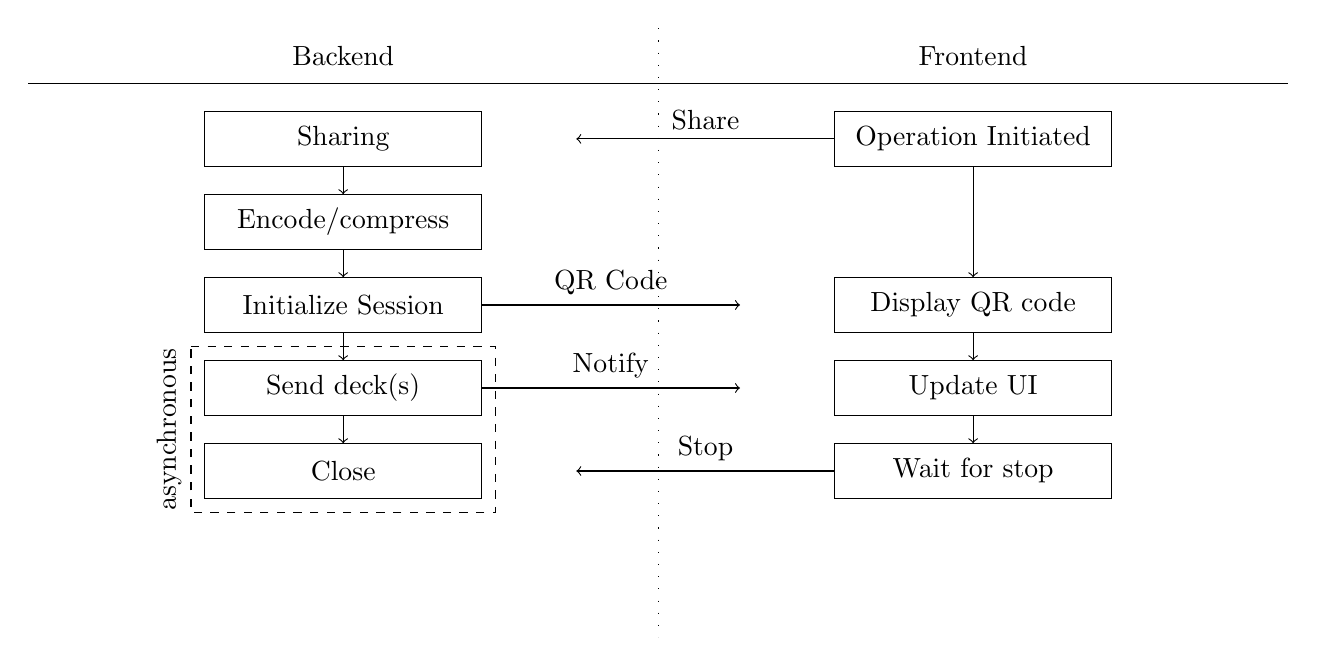
\begin{tikzpicture}
        \draw (0,0) -- (16,0);
        \draw[loosely dotted] (8,2em) -- (8,-20em);
        \draw (4,1em) node {Backend}
              (12,1em) node {Frontend};
        \node (Bsharing)    at (4,-2em)  [draw,minimum height=2em,minimum width=10em] {Sharing};
        \node (Bencode)     at (4,-5em)  [draw,minimum height=2em,minimum width=10em] {Encode/compress};
        \node (Bsessinit)   at (4,-8em)  [draw,minimum height=2em,minimum width=10em] {Initialize Session};
        \node (Bsenddeck)   at (4,-11em) [draw,minimum height=2em,minimum width=10em] {Send deck(s)};
        \node (Bclose)      at (4,-14em) [draw,minimum height=2em,minimum width=10em] {Close};
        \node (Finit)       at (12,-2em)  [draw,minimum height=2em,minimum width=10em] {Operation Initiated};
        \node (Fqrui)       at (12,-8em)  [draw,minimum height=2em,minimum width=10em] {Display QR code};
        \node (Fnotified)   at (12,-11em)  [draw,minimum height=2em,minimum width=10em] {Update UI};
        \node (Fstopped)    at (12,-14em) [draw,minimum height=2em,minimum width=10em] {Wait for stop};

        \draw[->] (Finit) ++(0,-1em) -- ++(0,-4em);
        \draw[->] (Fqrui) ++(0,-1em) -- ++(0,-1em);
        \draw[->] (Fnotified) ++(0,-1em) -- ++(0,-1em);

        \draw[->] (Bsharing) ++(0,-1em) -- ++(0,-1em);
        \draw[->] (Bencode) ++(0,-1em) -- ++(0,-1em);
        \draw[->] (Bsessinit) ++(0,-1em) -- ++(0,-1em);
        \draw[->] (Bsenddeck) ++(0,-1em) -- ++(0,-1em);

        \draw[->] (Finit) ++(-5em,0) -- ++(-9.34em,0) node[pos=0.5,above]{Share};
        \draw[->] (Bsessinit) ++(5em,0) -- ++(9.34em,0) node[pos=0.5,above]{QR Code};
        \draw[->] (Bsenddeck) ++(5em,0) -- ++(9.34em,0) node[pos=0.5,above]{Notify};
        \draw[->] (Fstopped) ++(-5em,0) -- ++(-9.34em,0) node[pos=0.5,above]{Stop};

        \draw[dashed] (Bsenddeck) ++(-5.5em,1.5em) -- ++(11em,0)
                                                   -- ++(0, -6em)
                                                   -- ++(-11em,0)
                                                   -- cycle
                                                   node[pos=0.5,above,rotate=90]{asynchronous};
    \end{tikzpicture}
\end{figure}

\section{Sharing flow between server and client devices}

\section{QR Code format}

\section{Network protocol}

\section{Security and Authentication}

\end{document}
